\documentclass[a4paper,11pt]{article}
\usepackage[top=2cm,bottom=2cm,left=2cm,right=2cm,asymmetric]{geometry}
\usepackage{url}
\usepackage{paralist}
\usepackage{authblk}
\usepackage{graphicx}
\usepackage[pdftex,colorlinks=true,hyperfootnotes=false]{hyperref}

\title{\vspace{-4em}A System for Automating Reproducibility in Science}

\author[1]{Tom Crick}
\author[2]{Benjamin A. Hall}
\author[3]{Samin Ishtiaq}
\affil[1]{Department of Computing \& Information Systems, Cardiff Metropolitan University}
\affil[2]{MRC Cancer Unit, University of Cambridge}
\affil[3]{Microsoft Research Cambridge}
\affil[1]{\protect\url{tcrick@cardiffmet.ac.uk}}
% \affil[2]{\protect\url{bh418@mrc-cu.cam.ac.uk}}
% \affil[3]{\protect\url{samin.ishtiaq@microsoft.com}}


\renewcommand\Authands{ and }
\def\UrlBreaks{\do\/\do-}

\date{ }

\begin{document}
\maketitle

\begin{abstract}
Need a short abstract here, 100 words...
\end{abstract}


%\vspace{-1.5cm}
\subsection*{Summary}

Reproducibility (replication, repeatability) is a basic tenet of good
science. This tenet holds all the more for digital science, with its
fundamentally more concrete outputs of algorithms and models. However,
there remain cultural and technical barriers to the sharing (using,
repeating, comparing, contributing, reimplementing) of these
artefacts, all the way from disseminating academic
publications~\cite{deroure:2010,stodden-et-al:2013,fursin+dubach:2014},
through to recognition of the importance of scientific
software~\cite{goble:2014} and computation~\cite{gent:2013}.

We believe that an automated notify+reproduce system, which allows
easy reproduction of the results of algorithms running on models, will
help significantly with lifting the cultural burden and, by doing so,
will vastly improve the efficiency of scientific exploration. Our
Digital Science Catalyst Grant proposal builds on this belief. While
there has been significant academic and policy discussion in this
space over the past few years, now is the time for the creation of an
extensible and adaptable open infrastructure to facilitate the
automation of science reproducibility.


\subsection*{Description}
{\textbf{We propose to develop a prototype open software platform
which will automate reproducibility for algorithms and models.}}  By
developing a cloud-based, centralised service, which performs
automated code compilation, testing and benchmarking, we will link
together published implementations of algorithms and input
models. This will allow the future extension of the prototype to link
together software and data repositories, toolchains, workflows and
outputs, providing a seamless automated infrastructure for the
verification and validation of scientific models and in particular,
performance benchmarks. The program of work will lead the cultural
shift in both the short- and long-term to move to a world in which
computational reproducibility helps researchers achieve their goals,
rather than being perceived as an overhead.

A system as described here has several up-front benefits: it links
papers more closely to their outputs, making external validation
easier and allows interested users to explore unaddressed sets of
models. Critically, it helps researchers to be more productive, rather
than reproducibility being an overhead on their day-to-day work. In
the same way that tools such as GitHub make collaborating easier while
simultaneously allowing effortless sharing, we hope that we can design
and build a system that is similarly usable for sharing and testing
benchmarks online.

There are already several web services that can do aspects of this
things (for example, a repository for disseminating the computational
models associated with publications in the social and life
sciences~\cite{rollins-et-al:2014}), so a service that can integrate
most if not all of these features is feasible. Such a service would
then allow algorithms and models to evolve together, and be
reproducible from the outset.

In summary, this proposed new infrastructure, previously highlighted
and discussed by the
authors~\cite{crick-et-al_wssspe2,crick-et-al_recomp2014}, would have
a profound impact on the way that open computational science is
performed, repositioning the role of models, algorithms and benchmarks
and accelerating the research cycle, perhaps truly enabling a ``fourth
paradigm'' of data intensive scientific
discovery~\cite{hey:2009}. Furthermore, it would effect the vital
cultural change by reducing overheads and improving the efficiency of
researchers.

\subsection*{Vision, Objective and Goals}

In the software development world, no one would (or should!) commit to
a project without first running the smoke tests. You could be clever
and run the tests via the version control system's pre-commit
hook. That way you would never forget to run the tests. All of this
can be done, at scale, on the cloud now. Services such as Visual
Studio Online\footnote{\url{http://www.visualstudio.com/en-us/products/what-is-visual-studio-online-vs.aspx}}
and Jenkins\footnote{\url{http://jenkins-ci.org/}}, etc, schedule the
tests to run as soon as you commit. We envisage moving to a world in
which benchmarks become available online, in the same vein as open
access of publications and research data. It seems a small step to
hook these continuous integration (CI) systems up to the algorithm
implementations that are written to run on these benchmarks.

Suppose you have come up with a better algorithm to deal with some of
these benchmarks. You write up the paper on the algorithm but, more
importantly, you also register the implementation of your algorithm at
this open service, as a possible algorithm to run on this benchmark
set. The benchmarks live in distributed git 
repositories. Some of the servers that house these repositories are CI
servers. Now, when you push a commit to your algorithm, or someone
else pushes a commit to theirs, or when someone else adds a new
benchmark, the service's CI system is triggered. It is also activated
with the addition of a new library, firmware upgrade, API change,
etc. All registered algorithms are run on all registered models, and
the results are published. The CI servers act as an authoritative
source, analogous to the Linux Kernel
Archives\footnote{\url{https://www.kernel.org/}}, of results for these
algorithms running on these benchmarks.

\subsection*{Workflow}

\begin{figure}[!h]
\centering
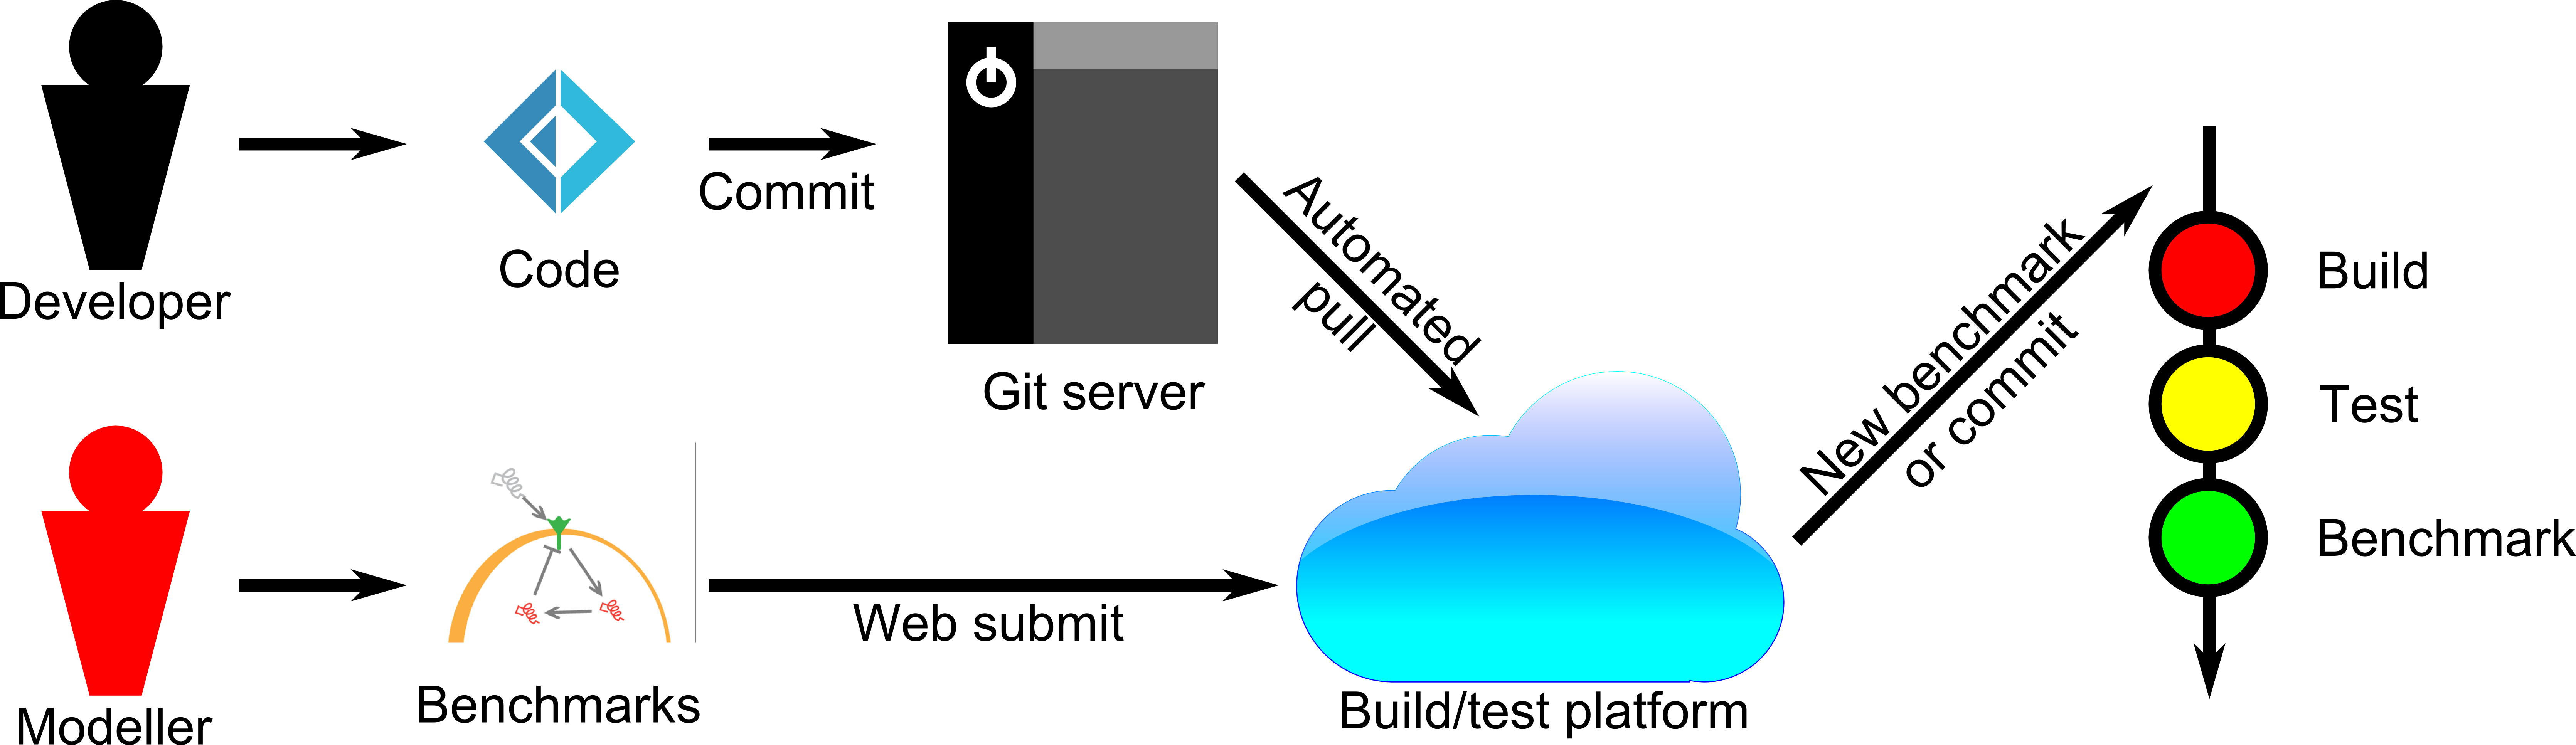
\includegraphics[width=\columnwidth]{workflow.png}
\caption{Proposed CI system workflow.}
\label{fig:workflow}
\end{figure}

The objective of this proposal is to develop a system which, through
integration with publicly available source code repositories automates
the build, testing and benchmarking of algorithms and benchmarks. The 
system will allow testing models against competing algorithms, and the
addition of new models to the test suite (either manually or from existing
online repositories). The goals are to:

\begin{itemize}
	\item Build a webserver, running a daemon which automatically pulls, and compiles
code from git repositories;
\item Run automated tests defined by the developers on the code;
\item Perform analysis of benchmark sets supplied by both the developer and external
users.
\item Work with key stakeholders in the open software/open data/open access/open
  science space, as well as key e-infrastructural organisations
  e.g. Digital Science, GitHub, figshare, Software Sustainability
  Institute, Mozilla Science Lab, etc.
\end{itemize}

This will be achieved over a period of six months, including regular
meetings for the design and requirements of the tool, and will involve
the employment of a dedicated programmer to implement the system.

% what do we need?
\subsection*{Resources}

% how will be push this to the research community?
\subsection*{Dissemination and Impact}

% may not need this, but worth showing our background and respective networks
\subsection*{Team Profile}

Dr Tom Crick\footnote{\url{http://drtomcrick.com}} is a Senior Lecturer in
Computing Science at Cardiff Metropolitan University, having completed
his PhD and post-doctoral research at the University of Bath. His
research interests cut across computational science: knowledge
representation and reasoning, intelligent systems, big data analytics,
optimisation and high performance computing.  He is the Nesta Data
Science Fellow, a 2014 Fellow of the Software Sustainability Institute
(EPSRC) and a member of {\emph{HiPEAC}}, the European FP7 Network of
Excellence on High Performance and Embedded Architecture and
Compilation.

% mention something about previous Azure work with Jasmine?
Dr Benjamin A. Hall\footnote{\url{http://www.mrc-cu.cam.ac.uk/hall.html}}
is a Royal Society University Research Fellow, developing hybrid and
formal models of carcinogenesis and biological signalling at the MRC
Cancer Unit, University of Cambridge. He previously worked at
Microsoft Research (Cambridge), UCL and the University of Oxford. As
part of his role at Oxford, he was one of two Apple
Laureates, awarded by Apple and the Oxford Supercomputing Centre for
the project {\emph{A biomolecular simulation pipeline}}. Benjamin has an
MBiochem and DPhil from the University of Oxford.

Dr Samin
Ishtiaq\footnote{\url{http://research.microsoft.com/en-us/people/sishtiaq/}}
is Principal Engineer in the Programming Principles and Tools group at
Microsoft Research Cambridge. He currently works on the SLAyer
(Separation Logic-based memory safety for C programs), TERMINATOR
(program termination) and BMA (analysis of gene regulatory networks)
projects. Samin joined MSR in April 2008. Before that (2000-2008), he
worked in CPU modelling and verification at ARM, helping to tape-out
the Cortex A8, Cortex M3 and SC300 processors, and the AMBA bus
protocol checker. Samin has an MEng from Imperial and a PhD in
dependent type theory from Queen Mary.

\bibliographystyle{unsrt}
\bibliography{Azure4Research}

\end{document}
